\section{Model}
\label{sec:model}

\subsection{CNN for Text Classification}

We propose a deep neural model to capture linguistics patterns in text. This model is based on Convolutional Neural Networks with an embedding layer for word representations, one convolutional with pooling layer and non-linearities. Finally we have two fully-connected layers. The final output size corresponds to the number of classes we attempt to train. The model is trained by cross-entropy with an Adam optimizer. Figure \ref{cnn} shows the global structure of our architecture. The input is a sequence of words $ w_{1}, w_{2} ... w_{n} $ and the output contains class probabilities (for text classification). The embedding is built on top of a Word2Vec architecture trained on a Skip-gram model. Our text tokenizer keeps all the words to make sure all linguistic material is detected at the end by the model. This embedding is also finetuned by the model to attain optimal text-classification accuracy. 

The Convolutional layer is based on a two-dimensional convolution, the same as used for image convolution, but with a fixed width equal to the embedding size. Indeed, word embeddings are not intended to hold spatial information. With this setting, our usage of the two-dimensional convolution is in reality the same as a one-dimensional convolution (the default settings for text). The only parameter we adjust here is the height of the filter corresponding to the number of words we want to put in the filter. 

they can be easily parallelized and may also be be easily used by the CPU, which is a practical solution for avoiding the use of GPUs at test time and thus providing wider access to our tools.

%The goal of this approach is to be able to use the standard image deconvolution (also called transposed convolutions) for our model on text.

\begin{figure}[h]
\begin{center}
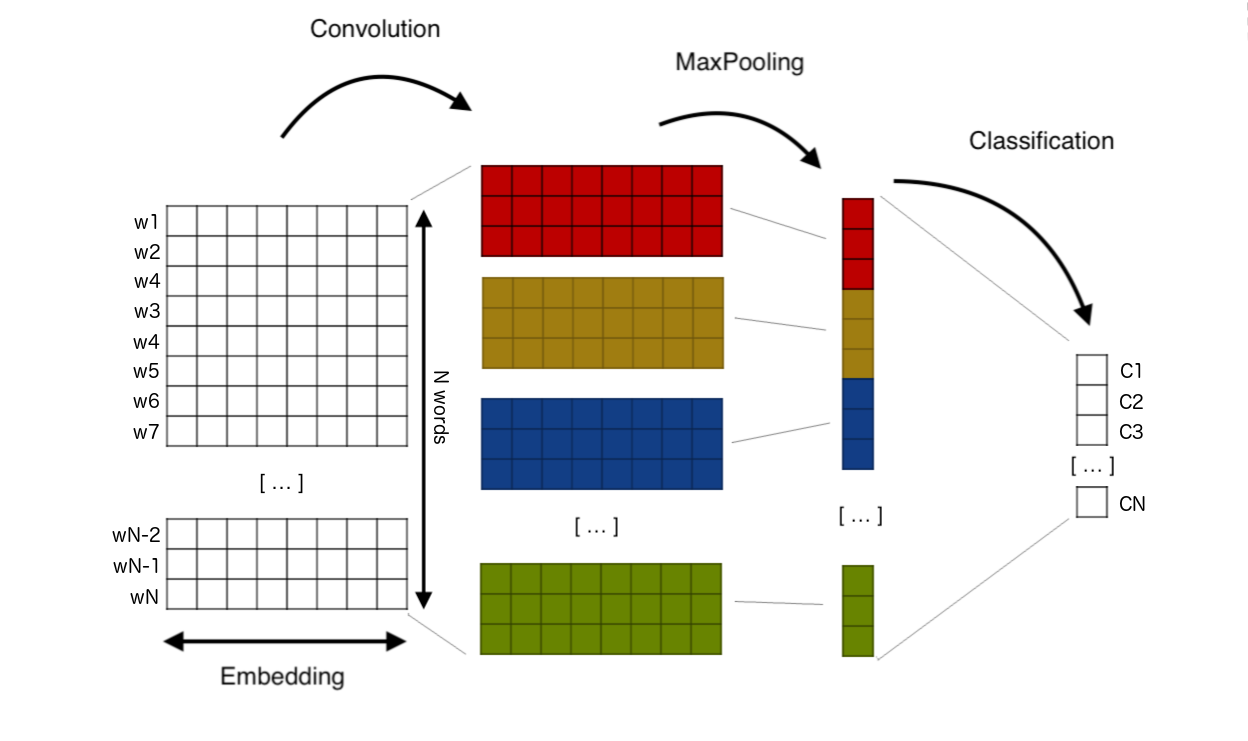
\includegraphics[width=8cm]{img/model_classif.png}
\caption{CNN model}
\label{cnn}
\end{center}
\end{figure}

\subsection{Deconvolution}

Since we use same architecture as image detection, making a deconvolutional layer is really straightforward. There are several methods to visualize the deep internal mecanisms of a neural network. One is known as convolutional transposed. Our deconvolutional network use the same embedding and convolution layer as we use for the classification but we replace the finale dense layer by a transposed convolution layer. After we trained the model we setup the weight of each neuron of the deconvolutional network with the learned weights of the classification network. The result is a new network that takes as input a sequence of words and gives as output all the trained filters of the text classification applied on the given sequence. Then the activation score of each word is calculated as shown in Equation \ref{equation} with $x$ is the size of the embedding, and $y$ the number of applied filters : 

\begin{equation}
\mathop{\sum^{x}\sum^{y}}_{i=1  j=1}  a_{ij} = s_{n}
\label{equation}
\end{equation}

\begin{figure}[h]
\begin{center}
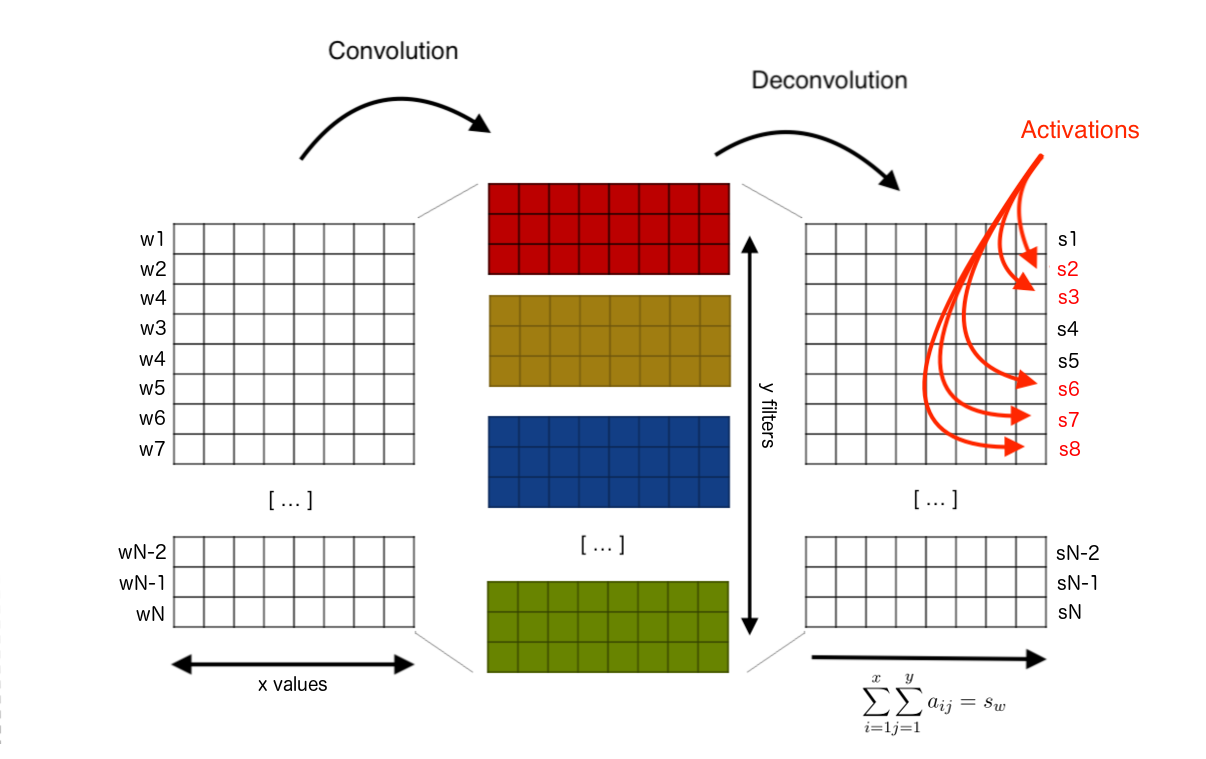
\includegraphics[width=8cm]{img/model_deconv.png}
\caption{Deconvolution model}
\label{cnn}
\end{center}
\end{figure}

With this method we are able to show a sort of topology of a sequence of words. All words have an unique activation score related to the others. We will see now that this output of the deconvolution gives us much information on how the network makes its final descision (prediction). There are well known linguistic marks encoded inside the networm, as well as more complex patterns based on co-occurrences and possibly also on grammatical and syntaxic analysis.
